\documentclass[uplatex, 12pt, dvipdfmx, twocolumn]{jsarticle}
\title{各種フォント}
\author{}
\date{}
\pagestyle{empty} \setcounter{secnumdepth}{4}
\input{/Users/hirofumi.shiba48/Desktop/数理科学/preamble_CM.tex}
\begin{document}
\maketitle

Computer Modern:
\begin{figure}[h]\centering
    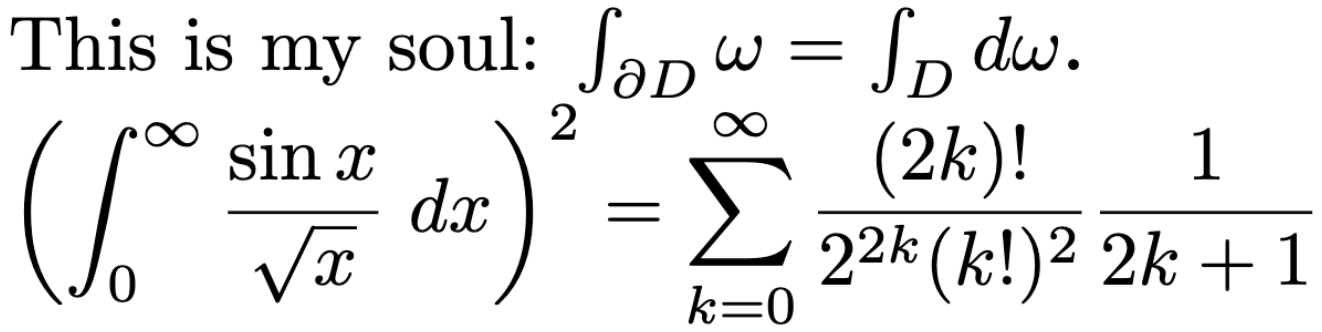
\includegraphics[width=7cm]{CM.png}
\end{figure}

mathpazo:
\begin{figure}[h]\centering
    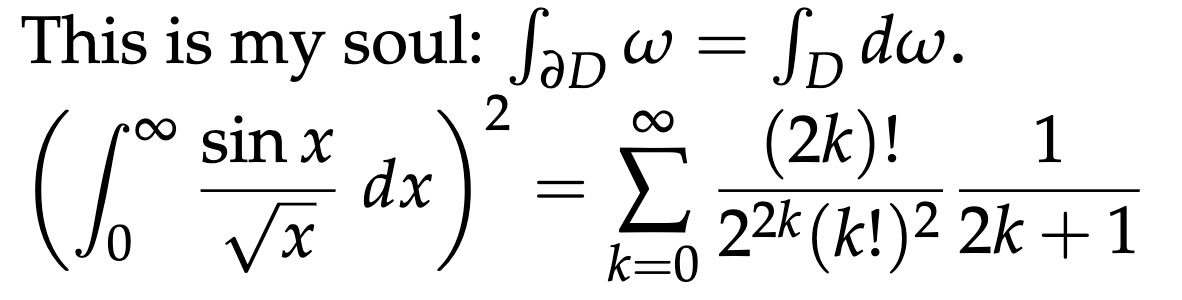
\includegraphics[width=7cm]{mathpazo.png}
\end{figure}

new txfonts:
\begin{figure}[h]\centering
    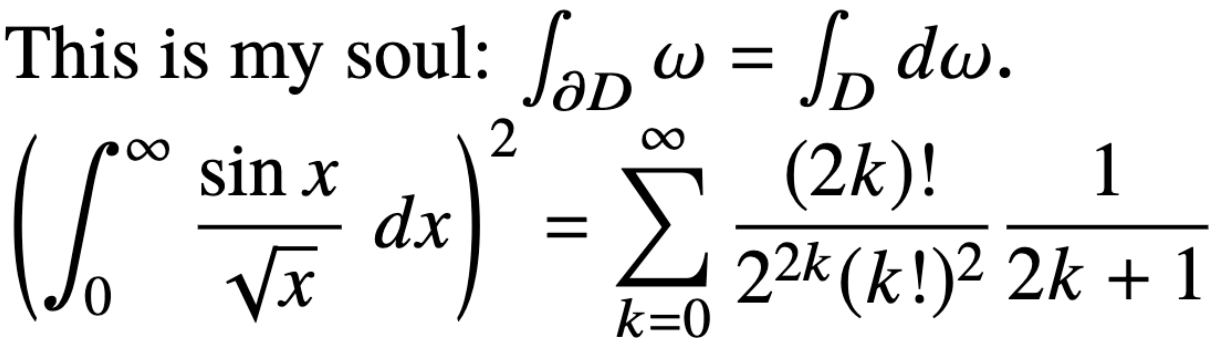
\includegraphics[width=7cm]{tx.png}
\end{figure}

Utopia:
\begin{figure}[h]\centering
    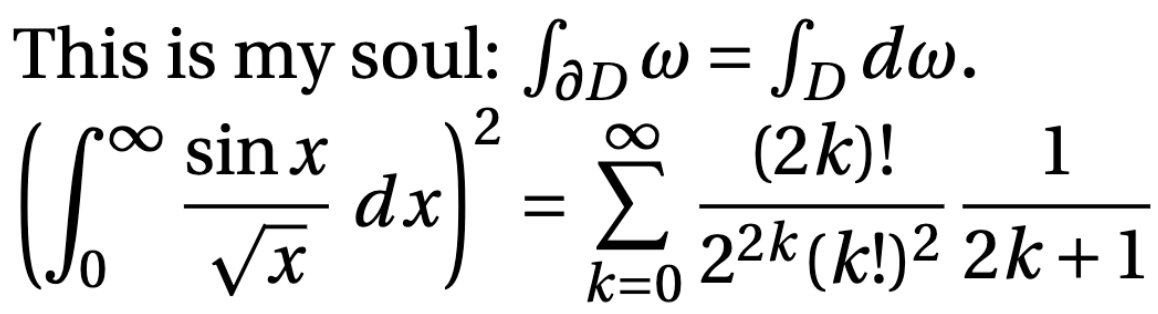
\includegraphics[width=7cm]{utopia.png}
\end{figure}

fouriernc:
\begin{figure}[h]\centering
    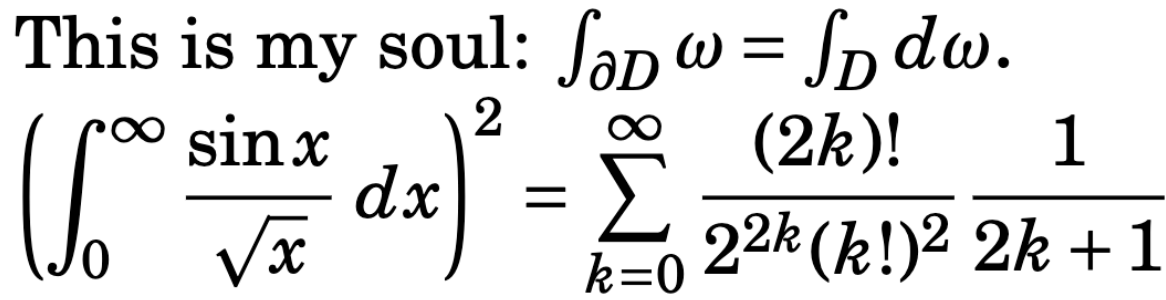
\includegraphics[width=7cm]{fnc.png}
\end{figure}

\newpage

Arev Sans fonts:
\begin{figure}[h]\centering
    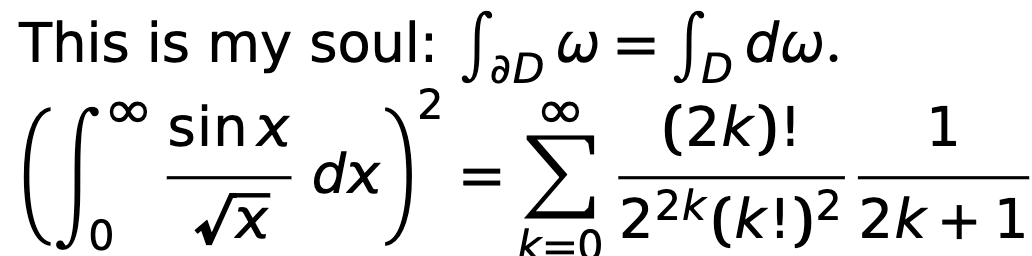
\includegraphics[width=7cm]{arev.png}
\end{figure}

CM Bright:
\begin{figure}[h]\centering
    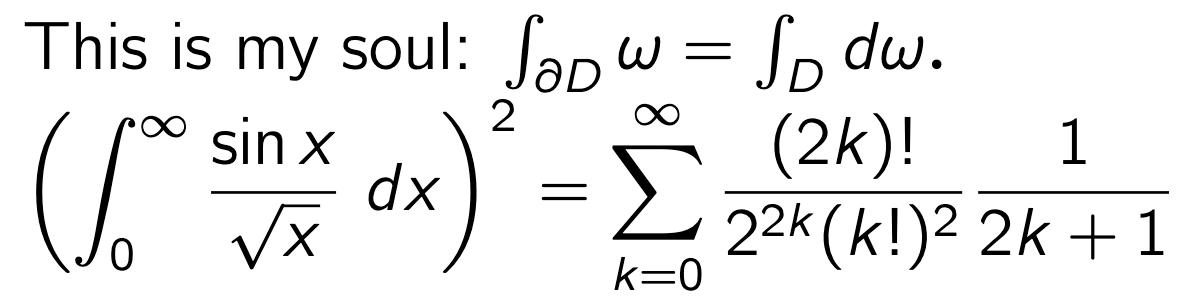
\includegraphics[width=7cm]{cmb.png}
\end{figure}

LX fonts:
\begin{figure}[h]\centering
    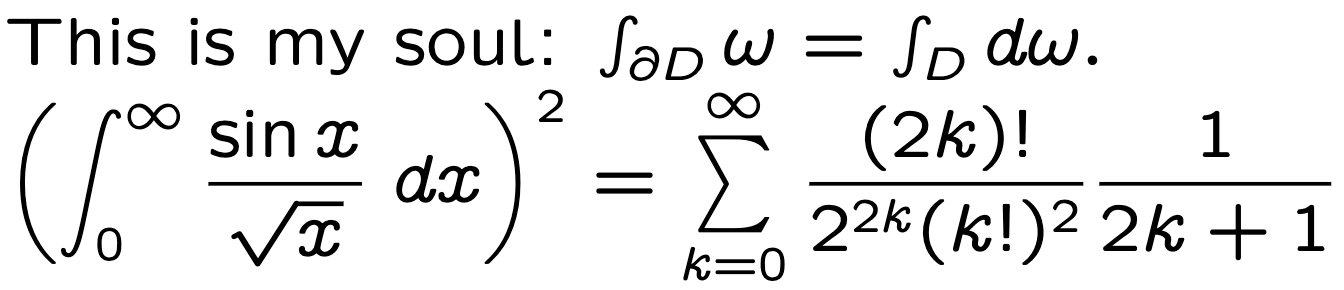
\includegraphics[width=7cm]{lx.png}
\end{figure}

Antiqua Toru\'{n}ska:
\begin{figure}[h]\centering
    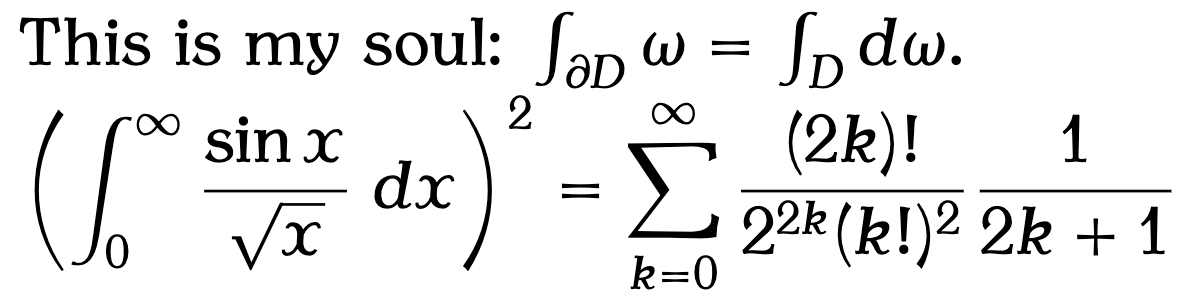
\includegraphics[width=7cm]{anttor.png}
\end{figure}

Concrete mathematics and Eular fonts:
\begin{figure}[h]\centering
    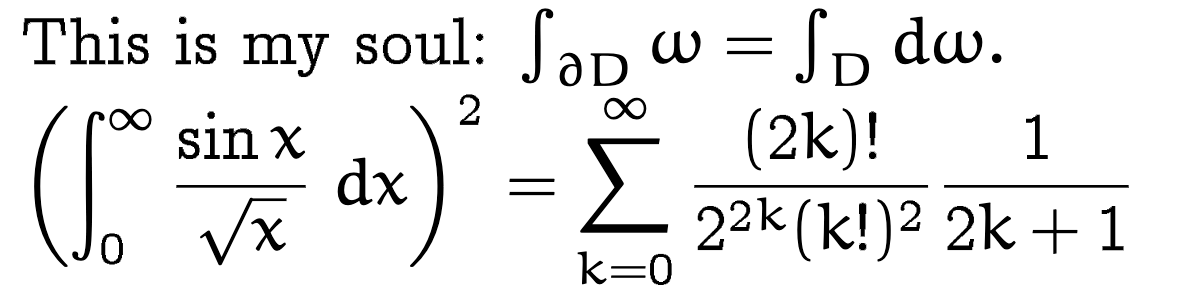
\includegraphics[width=7cm]{CMEULAR.png}
\end{figure}

\end{document}